\documentclass[a4paper]{article}

%% Language and font encodings
\usepackage[english]{babel}
\usepackage[utf8x]{inputenc}
\usepackage[T1]{fontenc}
\usepackage{parskip}

%% Sets page size and margins
\usepackage[a4paper,top=3cm,bottom=2cm,left=3cm,right=3cm,marginparwidth=1.75cm]{geometry}

%% Useful packages
\usepackage{amsmath}
\usepackage{graphicx}
\usepackage{tabularx}
\usepackage[colorinlistoftodos]{todonotes}
\usepackage[colorlinks=true, allcolors=blue]{hyperref}
\usepackage{diagbox}
\usepackage{fancyhdr}
\usepackage{placeins}
\usepackage{listings}
 
\pagestyle{fancy}
\fancyhf{}
\fancyhead[LE,RO]{Quantitative Computational Finance Program}
\fancyhead[RE,LO]{John Von Neumann Institute}
\fancyfoot[CE,LO]{Time Series Analytics and Forecasting}
\fancyfoot[LE,RO]{\thepage}
 
\renewcommand{\headrulewidth}{1pt}
\renewcommand{\footrulewidth}{1pt}

\begin{document}

\begin{titlepage}

\newcommand{\HRule}{\rule{\linewidth}{0.5mm}} % Defines a new command for the horizontal lines, change thickness here

\center % Center everything on the page
 
%----------------------------------------------------------------------------------------
%	HEADING SECTIONS
%----------------------------------------------------------------------------------------

\textsc{\LARGE John Von Neumann Institute}\\[1.5cm] % Name of your university/college
\textsc{\Large Quantitative Computational Finance Program}\\[0.5cm] % Major heading such as course name
\textsc{\large 2017 - 2019}\\[0.5cm] % Minor heading such as course title

%----------------------------------------------------------------------------------------
%	TITLE SECTION
%----------------------------------------------------------------------------------------

\HRule \\[0.4cm]
{ \huge \bfseries Time Series Analytics and Forecasting}\\[0.5cm] 
{ \huge \bfseries Project Report}\\[0.4cm] 
% Title of your document
\HRule \\[1.5cm]
 
%----------------------------------------------------------------------------------------
%	AUTHOR SECTION
%----------------------------------------------------------------------------------------

\begin{minipage}{0.4\textwidth}
\begin{flushleft} \large
\emph{Students:}\\
Valentine \textsc{CURE}\\ % Your name
Long \textsc{NGUYEN}
\end{flushleft}
\end{minipage}
~
\begin{minipage}{0.4\textwidth}
\begin{flushright} \large
\emph{Supervisors:}\\
\emph{Prof.:} Dr. Monique \textsc{PONTIER}\\ % Supervisor's Name
\emph{T.A.:} MSc. Tai T. \textsc{NGUYEN}
\end{flushright}
\end{minipage}\\[3cm]

% If you don't want a supervisor, uncomment the two lines below and remove the section above
%\Large \emph{Author:}\\
%John \textsc{Smith}\\[3cm] % Your name

%----------------------------------------------------------------------------------------
%	DATE SECTION
%----------------------------------------------------------------------------------------

{\large May 2018}\\[2cm] % Date, change the \today to a set date if you want to be precise

%----------------------------------------------------------------------------------------
%	LOGO SECTION
%----------------------------------------------------------------------------------------


\includegraphics[width=0.4\columnwidth]{jvnlogoh.png}\\[1cm] % Include a department/university logo - this will require the graphicx package
 
%----------------------------------------------------------------------------------------

\vfill % Fill the rest of the page with whitespace

\end{titlepage}
\newpage
\begin{abstract}
The Financial Time Series Analysis has a long history in the financial mathematics area with a vast amount of findings and methods in explanatory and forecasting. This report will mainly focus on the ARMA and GARCH modeling with the CAC 40 financial data, which is provided by Yahoo Finance. There are two main sections of the report which are the Theoretical Overview and the Case Study. The first part will be considered as a slight revision of the mandatory theory of Financial Time Series like the definition of Stationarity, Autocorrelation, ARCH model, GARCH model, etc. The second part would be the application of those theories on the CAC 40 financial data. Additionally, with the supporting of advanced development of R programming language, which has led to a faster calculation and fitting parameters of the model, the application section has smoothly gone through several stages such as data manipulation, visualizations, ARMA model fitting, ARMA residuals checking, GARCH model fitting. In short, the project report has illustrated a journey from mathematic logical proofs with computer programming support to figure out the real-life application on the CAC 40 stock market. 
\end{abstract}

\newpage
\tableofcontents
\newpage
\section{Theoretical Overview}
\label{sec:Theoretical}
\subsection {Introduction about Time Series Analysis}
A time series is a series of data, which was marked under an order of time.

The goal of quantitative researchers is to identify trends, seasonal variations and correlation in financial data using statistical time series methods, and ultimately generate trading signals. In order to improve the profitability of our trading models, we must make use of statistical techniques to identify consistent behavior in assets which can be exploited to turn a profit. To find this behavior, we must explore how the properties of the asset prices themselves change in time.

Time Series Analysis helps us to achieve this. It provides us with a robust statistical framework for assessing the behavior of time series, such as asset prices, in order to help us trade off of this behavior. Furthermore, the core theories of this part mainly rely on Pontier (2017) \cite{MPontier}, Tsay (2014) \cite{tsa2012} and Athanasopoulos and Hyndman (2013) \cite{hyndman2014forecasting} with detailed explanations. 

\subsection {Stationarity, Autocorrelation and White Noise}
		\subsubsection{Stationarity}  
Stationarity is an extremely important aspect of time series - much of the analysis carried out on financial time series data involves identifying if the series we want to predict is stationary, and if it is not, finding ways to transform it such that it is stationary. 
          \begin{itemize}
          \item  Mean of a time series $x_t$ is $E(x_t)=\mu(t)$
          \item  Variance of a time series $x_t$ is $\sigma^2(t)=E[(x_t - \mu(t))^2]$ 
          \item  A time series is stationary in the mean if $\mu(t)=\mu$, i.e.mean is constant with time
          \item  A time series is stationary in the variance if $\sigma^2(t)=\sigma^2$, i.e. variance is constant with time
         \end{itemize}
In short, A stationary time series (TS) is simple to predict as we can assume that future statistical properties are the same or proportional to current statistical properties. Most of the models we use in TSA assume covariance-stationarity. This means the predictions of these models - means, variances, and correlations, are only reliable if the TS is stationary and invalid otherwise.

     	\subsubsection {Serial Correlation – Autocorrelation}
A time series model decomposes the series into three components: Trend, Seasonal/cyclical and Random

The random component is called the residual or error - the difference between our predicted value(s) and the observed value(s). Autocorrelation is when these residuals (errors) are correlated with each other. That is, if the error of the $i_{th}$ is dependent on errors of any of the terms $0 .. i-1$ before. Essentially, it tells us how sequential observations in a time series affect each other.
		\begin{itemize}
          \item  \textbf{ACF} \\
Formally, for a covariance-stationary time series, the autocorrelation $\rho_k$ for lag $k$ (the number of time steps separating two sequential observations), 
$$\rho_k = \frac{COV(x_t, x_{t - k})}{\sigma_x^2} = \frac{E[(x_t - \mu)(x_{t - k} - \mu)}{\sigma_x^2}$$ 
A significant value of $\rho_k$ indicates that the error of the $i_{th}$ is dependent on the previous k terms from ${i-k} .. {i-1}$. 
\\
          \item  \textbf{PACF} \\
Then the Partial Autocorrelation Function (PACF) is defined as:
$$r(k) = Cor(X_t,X_{t+k}|X_{t+1},...,X_{t+k-1})$$ 
The PACF of lag k is the conditional correlation of $X_t$ and $X_{t+k}$ conditioned on $X_{t+1},...,X_{t+k-1}$
        \end{itemize}

Briefly, Serial correlation is critical for the validity of our model predictions - The residuals (errors) of a stationary TS are serially uncorrelated by definition. It is critical we account for autocorrelation in our model otherwise the standard errors of our estimates for the parameters will be biased and underestimated, making any tests that we try to form using the model invalid In layman's terms, ignoring autocorrelation means we're likely to draw incorrect conclusions about the impact of the independent variables in our model.

        \subsubsection {White Noise}
        
A white noise process is a time series that has serially uncorrelated errors and the expected mean of those errors is equal to zero. This means that the errors(residuals) are completely drawn at random from some probability distribution, i.e it is independent and identically distributed (i.i.d.). 

If our time series model results in white noise residuals, it means we have successfully captured the underlying process and explained any form of correlation, only leaving errors(residuals) which are completely random. Our predicted values differ from the observed values only by a random error component that cannot be forecast or modeled.

Most of the time series analysis is literally trying to fit a model to the time series such that the residual series is indistinguishable from white noise.

     	\subsubsection {Random Walk}
        
A random walk is a time series model where the value of the time series variable increases or decreases (step up or down) with equal probability at each time step, that is the expected value of current observation is equal to the previous observation. It is formally defined below:

$$x_t=x_{t-1}+w_t$$ , where $w_t$ is a discrete white noise series.
$$E[x_t]=x_{t-1}$$

This means if the TS we are modeling is a random walk it is unpredictable, as they are literally random walks.

The significance of a random walk is that it is non-stationary because while the mean of a random walk is still zero, the covariance is actually time-dependent. In particular, the covariance is equal to the variance multiplied by the time. Hence, as time increases, so does the variance.
 
\subsection {Auto Regressive(AR) and Moving Average(MA)}
		\subsubsection {Autoregressive Models - AM(p)}
        
The autoregressive model is simply an extension of the random walk. It is essentially a regression model which depends linearly on the previous terms:
$$x_t = \alpha_1x_{t-1}+…+\alpha_px_{t-p}+w_t = \sum_{i=1}^{p} t_i\alpha_ix_{t-i}+w_t$$

This is an AR model of order "p", where $p$ represents the number of previous (or lagged) terms used within the model, $\alpha_i$ is the coefficient, and $w_t$ is a white noise term. Note that an AR(1) model with $\alpha_1$ set equal to 1 is a random walk!

One of the most important aspects of the AR(p) model is that it is not always stationary. The stationarity of a particular model depends upon the parameters. For example, an AR(1) model with $\alpha_1$ = 1 is a random walk and therefore not stationary.
\\
     	\subsubsection {Moving Average Models - MA(q)}
        
MA(q) models are very similar to AR(p) models. MA(q) model is a linear combination of past error terms as opposed to a linear combination of past observations like the AR(p) model. The motivation for the MA model is that we can explain "shocks" in the error process directly by fitting a model to the error terms. (In an AR(p) model these shocks are observed indirectly by using past observations) 

$$x_t=w_t+\beta_1w_{t-1}+…+\beta_qw_{t-q}$$ 

Where $w_t$ is white noise with $E(w_t)=0$ and variance $\sigma^2$

By definition, ACF $\rho_k$ should be zero for k>q.

\subsection {ARMA model}
		\subsubsection {Extended Autocorrelation Function - EACF}
        
According to \cite{tsa2012}, the ACF and PACF are not informative in determining the order of an ARMA model. Thus we should have to look at a new approach proposed by Tsay and Tiao (1984) that uses the extended autocorrelation function (EACF) to specify the order of an ARMA process. The basic idea of EACF is relatively simple. If we can obtain a consistent estimate of the AR component of an ARMA model, then we can derive the MA component. From the derived MA series, we can use ACF to identify the order of the MA component.
\\
The output of EACF is a two-way table, where the rows correspond to AR order p and the columns to MA order q. The theoretical version of EACF for an ARMA(1,2) model is given in Table 1. The key feature of the table is that it contains a triangle of “O” with the upper left vertex located at the order (1,2). This is the characteristic we use to identify the order of an ARMA process. In general, for an ARMA(p,q) model, the triangle of “O” will have its upper left vertex at the (p,q) position \\

\FloatBarrier
\begin{table}[!htbp]
	\centering
  \begin{tabular}{|l||*{8}{c|}}
  \hline
  \backslashbox{AR}{MA}
  &\makebox[1em]{0}&\makebox[1em]{1}&\makebox[1em]{2}
  &\makebox[1em]{3}&\makebox[1em]{4}&\makebox[1em]{5}
  &\makebox[1em]{6}&\makebox[1em]{7} \\ 
  \hline\hline
  0 &*&X&X&X&X&X&X&X\\\hline
  1 &*&X&O&O&O&O&O&O\\\hline
  2 &*&*&X&O&O&O&O&O\\\hline
  3 &*&*&*&X&O&O&O&O\\\hline
  4 &*&*&*&*&X&O&O&O\\\hline
  5 &*&*&*&*&*&X&O&O\\\hline
  \end{tabular}
  \caption{Simplified table for EACF of an ARMA(1,2) model}
\end{table}
\FloatBarrier

The simplified table is constructed using the following notation:
\begin{enumerate}
\item “X” denotes that the absolute value of the corresponding EACF is greater than or equal to twice of its asymptotic standard error.
\item “O”  denotes  that  the  corresponding  EACF  is  less  than  twice  of  its  standard error in modulus.
\end{enumerate}
The  standard  error  of  EACF  can  be  computed  using  either  the  Bartlett’s formula,  or  simply  $2 / \sqrt{T}$ with $T$ being  the  sample  size (like \textit{TSA} package does with R). \\

		\subsubsection {Autoregressive Moving Average Models - ARMA(p, q)}
        
ARMA model is simply the merger between AR(p) and MA(q) models:
		\begin{itemize}
          \item  AR(p) models try to capture (explain) the momentum and mean reversion effects often observed in trading markets (market participant effects).
          \item  MA(q) models try to capture (explain) the shock effects observed in the white noise terms. These shock effects could be thought of as unexpected events affecting the observation process e.g. Surprise earnings, A terrorist attack, etc.
 		\end{itemize}
Hence, an ARMA model attempts to capture both of these aspects when modeling financial time series. Note that an ARMA model does not take into account volatility clustering, a fundamental empirical phenomenon of many financial time series which we will discuss later. 

$$x_t=\alpha_1x_{t-1}+…+\alpha_px_{t-p}+w_t+\beta_1w_{t-1}+…+\beta_qw_{t-q}$$ 

Where $w_t$ is white noise with $E(w_t)=0$ and variance $\sigma^2$

An ARMA model will often require fewer parameters than an AR(p) or MA(q) model alone. That is, it is redundant in its parameters

		\subsubsection {Information Criterion - AIC and BIC}

There are several information criteria available to determine orders (p,q) of an ARMA process. All of them are likelihood based. \\
When fitting models, it is possible to increase the likelihood by adding parameters, but doing so may result in overfitting. Both BIC and AIC criteria attempt to resolve this problem by introducing a penalty term for the number of parameters in the model. You will notice that the penalty term is larger in BIC than in AIC. \\
Akaike Information Criterion (AIC) (Akaike, 1973) is defined as
\begin{align}
AIC = 2k - 2ln(\hat{L})
\end{align}
where $\hat{L}$ is the maximized value of the likelihood function of the model and $k$ is  the number of estimated parameters in the model.
\\
The second term of the AIC in Equation (1) measures the
goodness of fit of the ARMA model to the data, whereas the first term is called the penalty function of the criterion because it penalizes a candidate model by the number of parameters used.
\\
Another  commonly  used  criterion  function  is  the  Schwarz – Bayesian  criterion (BIC, Bayesian information criterion).
\begin{align}
BIC = 2ln(n) - 2ln(\hat{L})
\end{align}
where $n$ is the the sample size, and other notations are the same as for AIC criterion.
\\
The penalty for each parameter used is 2 for AIC and $ln(n)$ for BIC.
Thus, compared with AIC, BIC tends to select a lower ARMA model when the sample size is moderate or large.

		\subsubsection {Other Model Accuracy Evaluation}
        \begin{itemize}
          \item  \textbf{Root Mean Square Error} \\
Given a series $y_1 , . . . , y_t$ and fitting a model and compute the forecasts $F_1 , . . . , F_t$ . The root mean square error of the model is
$$ RMSE = \sqrt{\frac{1}{t}\displaystyle\sum_{i=1}^{t}(y_i-F_i)^2} $$
In general, we will pick up the minimum RMSE value as it is equivalent with minimizing the mean square error (MSE)

          \item  \textbf{Mean Absolute Percent Error} \\
An alternative to RMSE, the mean absolute percent error is:
$$ MAPE = 100\frac{1}{t}\displaystyle\sum_{i=1}^{t}\mid \frac{y_i-F_i}{y_i}\mid $$
which takes into account the relative error in the prediction, rather than the absolute error. We also pick the lowest value of MAPE.
        \end{itemize}

\subsection {ARCH and GARCH models}
		\subsubsection {Conditional Heteroskedasticity}
        
The main motivation for studying Conditional Heteroskedasticity in finance is that of the volatility of asset returns.

A collection of random variables is heteroskedastic if there are certain groups, or subsets, of variables within the larger set that have a different variance from the remaining variables.

In finance, an increase in variance maybe correlated to a further increase in variance. For instance, on a day that equities markets undergo a substantial drop, automated risk management sell orders in long-only portfolios get triggered, which lead to further fall in the price of equities within these portfolios, leading to significant downward volatility.

These "sell-off" periods, as well as many other forms of volatility, lead to heteroskedasticity that is serially correlated and hence conditional on periods of increased variance. Thus we say that such series are conditional heteroskedastic.

One of the challenging aspects of conditional heteroskedastic series is ACF plots of a series with volatility might still appear to be a realization of stationary discrete white noise. This is even though the series is most definitely non-stationary as its variance is not constant in time.

To incorporate Conditional Heteroskedasticity in our model, we can create a model that utilizes an autoregressive process for the variance itself - a model that actually accounts for the changes in the variance over time using past values of the variance.

This is the basis of the Autoregressive Conditional Heteroskedastic (ARCH) model.
\\
     	\subsubsection {Autoregressive Conditionally Heteroskedastic - ARCH(p)}
ARCH(p) models can be thought of as simply an AR(p) model applied to the variance of a time series.

$$Var(\varepsilon_t) = \alpha_0 + \alpha_1Var(\varepsilon_{t-1})+…+\alpha_pVar(\varepsilon_{t-p})+w_t$$

The actual time series is given by:

$$\varepsilon_t = w_t\sqrt{\alpha_0 + \alpha_1\varepsilon_{t-1}^2+…+\alpha_p\varepsilon_{t-p}^2}$$

For ARCH(1), this reads:
$$\varepsilon_t = w_t\sqrt{\alpha_0+\alpha_1\varepsilon_{t-1}^2}$$

Furthermore, when we were attempting to fit an AR(p) model and are concerned with the decay of the pp lag on an ACF plot of the series, we can apply the same logic to the square of the residuals. If we find that we can apply an AR(p) to these square residuals, then we indicate that an ARCH(p) process may be appropriate.

Note that ARCH(p) should only ever be applied to a series that has already had an appropriate model fitted sufficient to leave the residuals looking like discrete white noise. Since we can only tell whether the ARCH is appropriate or not by squaring the residuals and examining the ACF, we also need to ensure that the mean of the residuals is zero.

ARCH should only ever be applied to series that do not have any trends or seasonal effects, i.e., that has no (evident) serially correlation. ARIMA is often applied to such a series, at which point ARCH may be a good fit.
\\
        \subsubsection {Generalized Autoregressive Conditionally Heteroskedastic - GARCH(p,q)}
GARCH(p, q)  is an ARMA model applied to the variance of a time series i.e., it has an autoregressive term and a moving average term. The AR(p) models the variance of the residuals (squared errors) or simply our time series squared. The MA(q) portion models the variance of the process.

$$\varepsilon_t = \sigma_t w_t$$

Where $w_t$ is discrete white noise, with zero mean and unit variance, and $\sigma^2$ is given by:

$$\sigma_t^2=\alpha_0+\sum_{i=1}^{p}\alpha_i\varepsilon_{t-i}^2+\sum_{j=1}^{q}\beta_j\sigma_{t-j}^2$$

Where $\alpha_i$ and $\beta_j$ are parameters of the model.For GARCH(1,1), $\sigma^2$ is:

$$\sigma_t^2=\alpha_0+\alpha_1\varepsilon_{t-1}^2+\beta_1\sigma_{t-1}^2$$

$\alpha_1 + \beta_1$ must be less than 1 or the model is unstable.
\\
		\subsubsection {Steps of ARCH/GARCH in Application:}
        \begin{itemize}
          \item  Iterate through combinations of ARIMA(p, d, q) models to best fit our time series.
          \item  Verify the ARCH Effect, Autocorrelation and Distribution of the Residual from ARIMA(p,d,q)
          \item  Pick the GARCH model orders according to the ARIMA model with lowest AIC/BIC.
          \item  Fit the GARCH(p, q) model to our time series.
          \item  Examine the model residuals and squared residuals for autocorrelation
        \end{itemize}

\label{sec:02Preliminarystudies}
\section{Preliminary studies}

\subsection{Data visualization}
We have worked on the closed price values of the CAC40 index as data, downloaded from the website finance.yahoo.com.\\
We started by displaying the data and trying to understand them, in order to be relevant in our way to study and model them.

\FloatBarrier
\begin{figure}[!htbp]
  \centering
  \includegraphics[width=\textwidth]{img/Plot1.eps}
  \caption{CAC40 values from 1998 to April 2018}
\end{figure}
\FloatBarrier

As we can see in the Figure 1, data seems to have a specific behavior during the period from 1998 to 2010, and a different evolution during the period from 2010 to 2018. In the first period indeed, data has known a high peak then a significant drop throughout 5-6 years, two times in a row, whereas in the second period they are just slightly increasing over time. \\
The drop which occurred in 2001 is because stock prices took a sharp downturn (some say "stock market crash" or "the Internet bubble bursting") in stock markets across the United States, Canada, Asia, and Europe. After recovering from lows reached following the September 11 attacks, indices slid steadily starting in March 2002, with dramatic declines in July and September leading to lows last reached in 1997 and 1998. \\
Regarding the drop from the middle of 2007, it can be explained by the global financial crisis of 2007-2008. \\
Given the fact that data evolution during the first period seems to be ruled by exceptional events, and the behavior or "stability" during the second one seems different, we decided to focus our work on data from 2012 to 2018 so our model will not be affected by events named above.

\FloatBarrier
\begin{figure}[!htbp]
  \centering
  \includegraphics[width=\textwidth]{img/Plot3.eps}
  \caption{CAC values from 2012 to April 2018, with train \& validation regions}
\end{figure}
\FloatBarrier

In practice, we have stored the data in a time series object, so we can use R’s many functions for analyzing time series data. We use the $ts()$ function in R to do that. \\
Since our time series data set has been collected at regular intervals, we specify the number of times that data was collected per year by using the $frequency$ parameter in the $ts()$ function. We set $frequency = 256$ since we have in average 256 data collected per year. \\
We also specify the first year that the data was collected, and the first interval in that year, by using the $start$ parameter in the $ts()$ function. Thus we set $start=c(2012,1)$. \\
We also set $end=c(2016,256)$ to work on data to the end of 2016, and thus we defined a period from 2012 to the end of 2016 to train our model, before testing it on the period from 2017 to 2018. It means that we will analyze how the model fit by comparing its forecast with the observed data over the period from 2017 to 2018 (the validation period), and only after this step we will perform forecasting.
 

\subsection{Data manipulation}
Our dataset leads us to reformat dates (from French to American format), and to remove null values and outliers. \\
Sometimes indeed we may have some outliers in our data, or simply null values, which can bring errors through analyses. To figure this out, we can use the $tsclean()$ function to detect and remove them. Here, we have manually removed null values in the data file, and comparison between data before and after the use of $tsclean()$ shows that there is apparently no outliers. \\


\subsection{Summary}
We can easily access to some statistical information about the serie, thanks to the R function summary(). Find in Tables 2 and 3 minimum, maximum and mean values, as well as the median and quartiles of our time series. \\

\FloatBarrier
\begin{table}[!htbp]
  \centering
  \begin{tabular}{|c c c|} 
  \hline
  Min. & Mean & Max. \\
  \hline
  2950 & 4386 & 5542 \\ 
  \hline
  \end{tabular}
  \caption{Mean and border values of the serie}
\end{table}
\FloatBarrier
\begin{table}[!htbp]
   \centering
   \begin{tabular}{|c c c|} 
   \hline
   1st Quart. & Median & 3rd Quart. \\
   \hline
   3982 & 4401 & 4911 \\ 
   \hline
  \end{tabular}
  \caption{Median and quartiles of the serie}
\end{table}
\FloatBarrier

\subsection{First analyses}
Following teacher's instruction, we used log transformation on the data.
Indeed, log transformation is usually used for several reasons :
\begin{enumerate}
\item to transform a multiplicative model to an additive model (see farther).
\item to remove unequal variances or exponential growth in the series.
\item in finance, for convenience (if price is log-normally distributed, or to approximate raw returns when returns are small, or for other mathematical and numerical advantages).
\end{enumerate}
However it might be not necessary here because as we can see with Figures 2 and 3, we have the same shape with and without the log transformation. \\

In Figure 3 we used \textit{lm()} function to carry out a regression, and \textit{abline()} function to plot it. \\
It shows that price is globally increasing over time, and also that this time series could probably be described using an \textbf{additive model}, since the random fluctuations in the data are roughly constant in size over time. \\
\\
\FloatBarrier
\begin{figure}[!htbp]
  \centering
  \includegraphics[width=\textwidth]{img/Fig3.eps}
  \caption{Log of the price}
\end{figure}
\FloatBarrier

\subsection{Data decomposition \& Stationarity}

\subsubsection{Additive and multiplicative models}
As we have seen in the first part of this report, ARMA modeling with time series requires series to be stationary. \\
We can deduce from Figure 3 that our series is not stationary, and the Augmented Dickey-Fuller Test \cite{banerjee1993co,said1984testing} with R confirms that we can't reject the null hypothesis of non-stationarity (p-value from the test is too high, see Listing 1). \\

\begin{lstlisting}[language=R, caption=First test of stationarity]
	Augmented Dickey-Fuller Test

data:  lserie
Dickey-Fuller = -2.5076, Lag order = 10, p-value =
0.3634
alternative hypothesis: stationary
\end{lstlisting}

To figure out this issue, we need to make some data transformations, like removing the seasonality, the trend, and/or differencing the serie. \\

Actually, time series are made up of four components:
\begin{enumerate}
  \item $S_t$: the seasonal component, which refers to fluctuations in the data related to calendar cycles.
  \item $T_t$: the trend component, which is the overall pattern of the series.
  \item $C_t$: the cyclical component, which consists of decreasing or increasing patterns that are not seasonal. Usually, trend and cycle components are grouped together. Trend-cycle component is estimated using moving averages (see farther).
  \item $E_t$: the error or irregular component, which is the part of the series which can't be attributed to other components.
\end{enumerate}
And we distinguish 2 kinds of decomposition for a time series :
\begin{enumerate}
  \item the additive decomposition: $Y_t = S_t + T_t + C_t + E_t$, where $Y_t$ is the data at time $t$.
  \item the multiplicative decomposition: $Y_t = S_t * T_t * C_t * E_t$.
\end{enumerate}

\subsubsection{Seasonality of the time series}
According to Figure X (above), there is no apparent seasonality in the data over this period, neither apparent cycle. Thus we could skip the seasonal adjustment and work on the trend of the time series. \\
On top of that, removing seasonality is not a mandatory step here, since with R we can build an ARMA model with orders (p,q) for the deseasonal part, and orders (P,Q) for the seasonal component. Such orders can be easily detected with the function \textit{auto.arima()}. \\
But for practice, this step will still be performed.

\subsubsection{Trend of the time series}
We can approach the trend component of our time series by taking successive orders of moving averages.\\
Note that the moving average in this context is distinct from the MA(q) component in the  ARIMA definition you have seen previously. Moving average MA(q) as part of the ARIMA framework refers to error lags and combinations, whereas the summary statistic of moving average refers to a data smoothing technique. \\
The wider the window of the moving average, the smoother original series becomes. In our case, we can take weekly, monthly or annual moving average, and then approximate the trend of the time series, as Figures 4 5 and 6 show.
\\
\FloatBarrier
\begin{figure}[!htbp]
  \centering
  \includegraphics[width=\textwidth]{img/Fig4.eps}
  \caption{Order 5 (weekly) moving average}
\end{figure}
\FloatBarrier
\FloatBarrier
\begin{figure}[!htbp]
  \centering
  \includegraphics[width=\textwidth]{img/Fig5.eps}
  \caption{Order 21 (monthly) moving average}
\end{figure}
\FloatBarrier
\FloatBarrier
\begin{figure}[!htbp]
  \centering
  \includegraphics[width=\textwidth]{img/Fig6.eps}
  \caption{Order 256 (annual) moving average}
\end{figure}
\FloatBarrier

\subsubsection{Decomposition of the time series}
With R, \textit{stl()} function allows us to decompose time series in 3 components :
\begin{enumerate}
  \item a seasonal component
  \item a trend-cycle component
  \item a remainder, or error component
\end{enumerate}

\FloatBarrier
\begin{figure}[!htbp]
  \centering
  \includegraphics[width=\textwidth]{img/Fig7.eps}
  \caption{Decomposition of the series}
\end{figure}
\FloatBarrier

As we can see in the Figure 7, the trend-cycle component looks like our approximation of the trend with moving averages (see Figure 6). \\
We also notice that the seasonal component is not null but very low compared with other components, and then it might be negligible, as we deduced before.\\

From now let's work with the log-transformed series as the time series under study. \\
We have two ways to remove seasonality from our time series:
\begin{enumerate}
\item Performing $Y_t^S = Y_t - S_t$, where $Y_t$ is the original data, and $S_t$ the seasonal component (because we have an additive model here, otherwise we would perform $\frac{Y_t}{S_t}$).
\item Using \textit{seasadj()} function from \textit{forecast} package, which removes the seasonal component given the result of the \textit{stl()} function as parameter.
\end{enumerate}
Both methods give the same result, available in Figure 8 \\

\FloatBarrier
\begin{figure}[!htbp]
  \centering
  \includegraphics[width=\textwidth]{img/Fig7b.eps}
  \caption{Deseasonalized Series}
\end{figure}
\FloatBarrier

For the trend component, we also have two ways to remove it :
\begin{enumerate}
\item Performing $Y_t^{S,T} = Y_t^S - T_t$, where $Y_t^S$ is the deseasonalized time series, and $T_t$ the trend component (here trend-cycle component).
\item Using function \textit{diff()}.
\end{enumerate}

With R, \textit{diff()} function returns, given a time series $(X)_t$ as parameter, a time series $(Z)_t$ which is the differences between all consecutive values of $(X)_t$. In other words, $Z_t = X_{t+1} - X_t$. If $(X)_t$ is not stationary but $(Z)_t$ is, then we can identify an ARMA($p_z$,$q_z$) model for $(Z)_t$, which will be an ARIMA($p_z$,$1$,$q_z$) for $(X)_t$. Indeed, each use of the \textit{diff()} transformation increments by 1 the order $d$. If it happens that $d=1$ is not enough to get a stationary series, then we try with higher values of $d$ until the series is stationary. \\
Here we decided to first try to remove the trend-cycle component of the deseasonalized series, before taking an interest in the differentiated series. The result is available in Figure 9 below.

\FloatBarrier
\begin{figure}[!htbp]
  \centering
  \includegraphics[width=\textwidth]{img/Fig7c.eps}
  \caption{Random Part of the Series}
\end{figure}
\FloatBarrier

\subsubsection{Stationarity of the decomposed time series}

From Figure 9, we can see that our series seems to be stationary, because data values oscillate with a steady variance around the mean of 0.
In addition, the Augmented Dickey-Fuller test with R confirms that we can reject the null hypothesis of non-stationarity since the p-value from the test is lower than 0.05 (Listing 2). \\

\begin{lstlisting}[language=R, caption=Final test of stationarity]
	Augmented Dickey-Fuller Test

data:  random_stl
Dickey-Fuller = -4.4514, Lag order = 10, p-value = 0.01
alternative hypothesis: stationary
\end{lstlisting}
\label{sec:03IdentifyARMAmodel}
\section{Identify ARMA model}
Now that our time series is stationary, we can determine values of p and q for our ARMA(p,q) model. Several methods exist to determine them. \\

\subsection{With auto.arima() function built-in R}
There is a built-in function in R which helps to determine values of $p$ and $q$ for an ARMA model. This is a first "automatic" result which will serve to do comparisons with our results. \\
Note that it also gives values of parameter d, and (P,D,Q) parameters for the seasonal part if it exists. \\
We have performed several tests with this function. \\
For example, 
\begin{lstlisting}[language=R]
auto.arima(data,seasonal=FALSE, stepwise=FALSE, approximation=FALSE)
\end{lstlisting}
forced \textit{auto.arima()} to run longer and with more trial/error testing cases, and selected an ARMA(3,2) model. \\
However 
\begin{lstlisting}[language=R]
auto.arima(data,seasonal=FALSE, stepwise=TRUE, approximation=TRUE)
\end{lstlisting} 
returned an ARMA(1,0) model.


\subsection{With extended autocorrelation function (EACF)}

Table 5 shows the sample EACF and Table 4 its corresponding simplified table for the series, obtained via the \textit{TSA} package.
\FloatBarrier
\begin{table}[!htbp]
	\centering
  \begin{tabular}{|l||*{11}{c|}}
  \hline
  \backslashbox{AR}{MA}
  &\makebox[1em]{0}&\makebox[1em]{1}&\makebox[1em]{2}
  &\makebox[1em]{3}&\makebox[1em]{4}&\makebox[1em]{5}
  &\makebox[1em]{6}&\makebox[1em]{7}&\makebox[1em]{8}
  &\makebox[1em]{9}&\makebox[1em]{10} \\
  \hline\hline
  0 &X&X&X&X&X&X&X&X&X&X&X\\\hline
  1 &O&O&X&O&X&X&O&O&O&O&O\\\hline
  2 &X&O&O&O&X&X&O&O&O&O&O\\\hline
  3 &X&X&O&O&X&X&O&O&O&O&O\\\hline
  4 &X&X&X&O&O&X&X&X&O&O&O\\\hline
  5 &X&X&X&X&O&X&O&O&O&O&O\\\hline
  6 &X&X&X&X&X&X&O&O&O&O&O\\\hline
  7 &X&X&O&X&X&O&X&O&O&O&O\\\hline
  \end{tabular}
  \caption{Simplified table for EACF}
\end{table}
\FloatBarrier
\FloatBarrier
\begin{table}[!htbp]
	\centering
  \begin{tabular}{|l||*{11}{c|}}
  \hline
  \backslashbox{AR}{MA}
  &\makebox[1em]{0}&\makebox[1em]{1}&\makebox[1em]{2}
  &\makebox[1em]{3}&\makebox[1em]{4}&\makebox[1em]{5}
  &\makebox[1em]{6}&\makebox[1em]{7} \\
  \hline\hline
0 & 0.960 & 0.9227 & 0.8884 & 0.8519 & 0.820 & 0.797 & 7.7e-01 & 0.7403 \\\hline
1 & -0.028 &-0.0150 & 0.0568 &-0.0438 &-0.099 &0.069 & 2.6e-02 & 0.0186  \\\hline
2& -0.426& -0.0087&  0.0288& -0.0277& -0.091 &0.091 &-1.5e-02& -0.0065  \\\hline
3&  0.260 & 0.3307 &-0.0052 &-0.0186 &-0.060& 0.094& -2.0e-02 &-0.0151 \\\hline
4 & 0.477 & 0.2467 &-0.2051& -0.0061& -0.046& 0.079 & 7.1e-02 & 0.0732 \\\hline
5 &-0.350 & 0.4322& -0.3204&  0.1046&-0.033& 0.081 &-1.7e-04 & 0.0342 \\\hline
6&  0.440&  0.3787&  0.3165&  0.3120  &0.244& 0.081 &-5.6e-05& 0.0269 \\\hline
7 &-0.419& -0.0716 &-0.0093&  0.1480 &-0.101& 0.010 &7.7e-02&  0.0304 \\\hline
  \end{tabular}
  \caption{EACF table}
\end{table}
\FloatBarrier

The simplified  table exhibits  a  triangular  pattern  of  “O”  with  its  upper  left  vertex  at  the  order  (p,q) = (1,0).
A few exceptions of “X” appear when q = 2, 4, 5, 6 and 7.
However, the EACF table  shows  that  the  values  of  sample  ACF  corresponding  to  those  “X”  are  around 0.08 or 0.09.
These ACFs are only slightly greater than $2 / \sqrt{1280} = 0.0559$. Indeed, if 3\% critical value is used, those “X” would become “O” in the simplified EACF table.
Consequently,  the  EACF  suggests  that  the  time series  follows an ARMA(1,0) model.


\subsection{With information criteria AIC \& BIC}

\subsubsection{Selection rule}
To use AIC to select an ARMA model in practice, one computes $AIC(i,j)$ for $i = 0,...,P$, $j = 0,...,Q$, where $P$ and $Q$ are prespecified positive integers and selects the orders $(p,q)$ that has the minimum AIC value.
\\
The same rule applies to BIC.
\\

\subsubsection{Results}
For our analysis, we obtain the following tables for AIC and BIC values.

AIC has a minimum value of -7979.095 for (p,q) = (7,7), and so would prefer an ARMA(7,7) model, whereas BIC would select an ARMA(1,0) model since it reaches its minimum value of -7940.592 for (p,q) = (1,0) \\

\underline{Remark:} We can notice that the value of AIC(3,2) is a local minimum in Table 5, and ARMA(3,2) was a potential candidate from \textit{auto.arima()} function. Therefore, this model could be a compromise, since it has a better AIC than ARMA(1,0) and less parameters than ARMA(7,7). \\

\FloatBarrier
\begin{table}[!htbp]
  \centering
  \begin{tabular}{|l||*{10}{c|}}\hline
\backslashbox{p}{q}
&\makebox[3em]{0}&\makebox[3em]{1}&\makebox[3em]{2}
&\makebox[3em]{3}&\makebox[3em]{4}&\makebox[3em]{5}
&\makebox[3em]{6}\\
\hline\hline
0 &-4663.050&-5956.074&-6675.836&-7041.741&-7375.061&-7509.821&-7595.880\\\hline
1 &-7956.056&-7955.018&-7953.200&-7954.187&-7955.289&-7963.993&-7967.363\\\hline
2 &-7955.005&-7953.072&-7952.094&-7952.759&-7951.573&-7965.143&-7967.512\\\hline
3 &-7953.304&-7952.396&-7961.873&-7961.244&-7959.894&-7964.671&-7965.805\\\hline
4 &-7955.051&-7953.458&-7961.332&-7959.371&-7960.121&-7962.767&-7960.667\\\hline
5 &-7955.061&-7952.697&-7959.003&-7959.599&-7972.342&-7971.264&-7973.164\\\hline
6 &-7965.151&-7965.741&-7964.712&-7963.150&-7971.495&-7970.143&-7968.482\\\hline
7 &-7967.376&-7968.029&-7966.036&-7964.594&-7971.115&-7975.143&-7967.147\\\hline
8 &-7966.607&-7966.032&-7964.029&-7969.871&-7971.906&-7969.088&-7967.039\\\hline
9 &-7965.696&-7964.296&-7978.027&-7974.690&-7964.050&-7968.126&-7979.055\\\hline
\end{tabular}
\caption{Table with AIC values (first part)}
\end{table}

\FloatBarrier
\begin{table}[!htbp]
  \centering
  \begin{tabular}{|l||*{10}{c|}}\hline
\backslashbox{p}{q}
&\makebox[3em]{7}&\makebox[3em]{8}&\makebox[3em]{9}\\
\hline\hline
0 &-7672.402&-7712.736&-7761.958\\\hline
1 &-7966.806&-7965.549&-7964.442\\\hline
2 &-7965.795&-7963.914&-7962.569\\\hline
3 &-7965.519&-7963.101&-7962.896\\\hline
4 &-7961.823&-7959.993&-7968.672\\\hline
5 &-7972.918&-7971.996&-7955.056\\\hline
6 &-7968.623&-7960.931&-7960.527\\\hline
7 &-7979.095&-7977.973&-7952.614\\\hline
8 &-7960.482&-7962.310&-7960.790\\\hline
9 &-7955.190&-7968.666&-7964.813\\\hline
\end{tabular}
\caption{Table with AIC values (second part)}
\end{table}

\FloatBarrier
\begin{table}[!htbp]
\centering
\begin{tabular}{|l||*{8}{c|}}\hline
\backslashbox{p}{q}
&\makebox[3em]{0}&\makebox[3em]{1}&\makebox[3em]{2}
&\makebox[3em]{3}&\makebox[3em]{4}&\makebox[3em]{5}
&\makebox[3em]{6}&\makebox[3em]{7} \\ 
\hline\hline
0 &-4652.740&-5940.610&-6655.217&-7015.968&-7344.134&-7473.738&-7554.643&-7626.010\\\hline
1 &-7940.5920&-7934.400&-7927.426&-7923.260&-7919.206&-7922.756&-7920.971&-7915.260\\\hline
2 &-7934.387&-7927.299&-7921.167&-7916.676&-7910.336&-7918.752&-7915.965&-7909.095\\\hline
3 &-7927.531&-7921.468&-7925.790&-7920.007&-7913.503&-7913.125&-7909.104&-7903.663\\\hline
4 &-7924.124&-7917.376&-7920.095&-7912.980&-7908.575&-7906.066&-7898.811&-7894.813\\\hline
5 &-7918.979&-7911.460&-7912.611&-7908.053&-7915.641&-7909.408&-7906.154&-7900.753\\\hline
6 &-7923.914&-7919.350&-7913.166&-7906.449&-7909.640&-7903.133&-7896.318&-7891.304\\\hline
7 &-7920.985&-7916.483&-7909.335&-7902.738&-7904.105&-7902.978&-7889.828&-7896.621\\\hline
\end{tabular}
\caption{Table with BIC values}
\end{table}
\FloatBarrier
This example shows that different approaches or criteria to order determination may result in different choices of $p$ and $q$. There is no evidence to suggest that one method outperforms the other in a real application. Substantive information of the problem under study and simplicity are two factors that also play an important role in choosing an ARMA model for a given time series.

\subsection{With ACF and PACF}

\FloatBarrier
\begin{figure}[!htbp]
  \centering
  \includegraphics[width=\textwidth]{img/Fig7d.eps}
  \caption{ACF of the Random Part of the Serie}
\end{figure}
\FloatBarrier
\begin{figure}[!htbp]
  \centering
  \includegraphics[width=\textwidth]{img/Fig7e.eps}
  \caption{PACF of the Random Part of the Serie}
\end{figure}
\FloatBarrier
We see from the correlogram (Figure 10) that the autocorrelations for many lags in a row exceed the significance bounds, are positive, decrease in magnitude with increasing lag, and tail off to zero after lag 40. Therefore the autocorrelation function shows significant autocorrelation. This does not necessarily mean the series is non-stationary, but it's telling us that the observations are not independent. \\
From the partial autocorrelogram (Figure 11), we see that the partial autocorrelation at lag 1 is positive and exceeds the significance bounds (0.96), while it tails off to zero after lag 1 (with some exceptions for lags 6, 7, and 25, but their excess is very low). Thus an AR(1) model seems possible for the time series.


\subsection{Conclusion}
According to our results, we decided to work with an ARMA(1,0) model, since it is the one selected by EACF method, BIC criterion, and $auto.arima()$ function. Other models that could have been selected are ARMA(7,7) for its best AIC value, or ARMA(3,2) to get a compromise between ARMA(1,0) and ARMA(7,7) as explained above.\\


Therefore, we deduce from the Listing 3, noting our time series $(X)_t$, that
\begin{align*}
X_t−0,0022 
 	&= 0,9621[X_{t-1}−0,0022] + W_t \\
\text{i.e.} \ X_t 
	&= 8,338.10^{-5} + 0,9621 X_{t-1} + W_t
\end{align*}
where $W_t$ is $\mathcal{N}(0,1)$ noise.
\begin{lstlisting}[language=R, caption=ARMA model]
Call:
arima(x = random_stl, order = c(1, 0, 0), seasonal = c(0, 0, 0))

Coefficients:
         ar1  intercept
      0.9621     0.0022
s.e.  0.0076     0.0078

sigma^2 estimated as 0.0001162:  log likelihood = 3981.03,  aic = -7956.06
\end{lstlisting}
\label{sec:04TheResidualsanalysis}
\section{The Residuals $\varepsilon_t^2 = (X_t - X_{t-1})^2$ analysis}
\subsection{Plotting}
We will plot the residuals and residual squared of ARMA(1,0) series
\FloatBarrier
\begin{figure}[!htbp]
  \centering
  \includegraphics[width=\textwidth]{img/Fig8.eps}
  \caption{The Residual plot}
\end{figure}
\FloatBarrier
\FloatBarrier
\begin{figure}[!htbp]
  \centering
  \includegraphics[width=\textwidth]{img/Fig9.eps}
  \caption{The Residual Squared plot}
\end{figure}
\FloatBarrier
\subsection{Distribution Checking}
In order to check the distribution, we first run $shapiro.test()$ function, which will run the Shapiro-Wilk Test \cite{royston1982extension} with following results:
\begin{lstlisting}[language=R, caption=Shapiro-Wilk normality test]
Shapiro-Wilk normality test
data:  Resids
W = 0.98495, p-value = 2.991e-10
\end{lstlisting}
The $H_0$: Normal Distribution \\
The $H_1$: Not Normal Distribution \\
The p-value is less than 0.05, so we can concluded that the Residuals are not distributed Normality. 

\FloatBarrier
\begin{figure}[!htbp]
  \centering
  \includegraphics[width=\textwidth]{img/Fig10.eps}
  \caption{The Normal Distribution QQ plot of ARMA residuals}
\end{figure}
\FloatBarrier
Then we will test with Student's t-distribution with $ks.test.t()$ function - based on Kolmogorov-Smirnov test \cite{dujrbin1973distribution}, and received following outcome:
\begin{lstlisting}[language=R, caption=Kolmogorov-Smirnov test student-t with df=7.42]
data:  fit1$residuals
D = 0.015544, p-value = 0.9166
\end{lstlisting}
The $H_0$: Student's t-distribution \\
The $H_1$: Not Student's t-distribution \\
The p-value is higher than 0.05, so we can concluded that the Residuals are Student's t-distribution. 

\FloatBarrier
\begin{figure}[!htbp]
  \centering
  \includegraphics[width=\textwidth]{img/Fig11.eps}
  \caption{The Student's t-distribution QQ plot of ARMA residuals}
\end{figure}
\FloatBarrier

\subsection{Autocorrelation Test}
We use the Box-Ljung Test \cite{box1970distribution,ljung1978measure}, which indicated in $Box.test()$ function to test the Autocorrelation of Residuals as following:
\begin{lstlisting}[language=R, caption=Box-Ljung test]
Box-Ljung test
data:  fit1$residuals
X-squared = 73.912, df = 50, p-value = 0.01559
\end{lstlisting}
The $H_0$: The residuals are independently distributed \\
The $H_1$: The residuals are not independently distributed \\
p-value less than 0.05 then reject the Null Hypothesis, which means the residuals are independently distributed.\\
The below ACF and PACF plots also support this conclusion
\FloatBarrier
\begin{figure}[!htbp]
  \centering
  \includegraphics[width=\textwidth]{img/Fig12.eps}
  \caption{ACF of ARMA(1,0) Residuals}
\end{figure}
\FloatBarrier
\FloatBarrier
\begin{figure}[!htbp]
  \centering
  \includegraphics[width=\textwidth]{img/Fig13.eps}
  \caption{PACF of ARMA(1,0) Residuals}
\end{figure}
\FloatBarrier

\subsection{ARCH Effect Verification}
We use the function $arch.test()$, which implement the Portmanteau Q and the Lagrange Multiplier test statistic \cite{mcleod1983diagnostic,engle1982autoregressive} in order to verify whether the Residuals got ARCH Effects. The result as follow:
\begin{lstlisting}[language=R, caption=ARCH Heteroscedasticity test for residuals]
ARCH heteroscedasticity test for residuals 
alternative: heteroscedastic 

Portmanteau-Q test: 
     order   PQ  p.value
[1,]     4 33.8 8.25e-07
[2,]     8 51.7 1.95e-08
[3,]    12 64.9 2.89e-09
[4,]    16 69.1 1.43e-08
[5,]    20 77.2 1.19e-08
[6,]    24 83.7 1.57e-08
Lagrange-Multiplier test: 
     order  LM  p.value
[1,]     4 755 0.00e+00
[2,]     8 373 0.00e+00
[3,]    12 232 0.00e+00
[4,]    16 172 0.00e+00
[5,]    20 132 0.00e+00
[6,]    24 108 5.45e-13
\end{lstlisting}
\FloatBarrier
\begin{figure}[!htbp]
  \centering
  \includegraphics[width=\textwidth]{img/Fig14.eps}
  \caption{The Student's t-distribution QQ plot of ARMA residuals}
\end{figure}
\FloatBarrier

From both Portmanteau-Q test and Lagrange-Multiplier test, with p.value significantly less than 0.05, we can concluded that the Residuals of ARMA(1,0) got ARCH Effect and lead to the applying of GARCH model for the Residuals. 
\label{sec:05IdentifyGARCHmodel}
\section{Identify GARCH model}
\subsection{Using \textit{garchFit()} function and AIC}

In this section, we will try to fit the Residuals into a GARCH model due to the previous test proved that there are existing an ARCH Effect on the Residuals. Similar to fitting the ARMA Model, we will mainly rely on the AIC to search the (p,q) figures, which resulted in the smallest value then verify back with BIC.

By using the $garchFit()$ function and fitting with (p,q) $\in$ $\{1,2,..7\}$. We generated the table of AIC:

\FloatBarrier
\begin{table}[!htbp]
\centering
\begin{tabular}{|l||*{8}{c|}}\hline
\backslashbox{p}{q}
&\makebox[3em]{1}&\makebox[3em]{2}&\makebox[3em]{3}&\makebox[3em]{4}&\makebox[3em]{5}&\makebox[3em]{6}&\makebox[3em]{7} \\
\hline\hline
1 &-6.291084&-6.26150&-6.26064&-6.25907&-6.25752&-6.25595&-6.25559\\\hline
2 &-6.26127&-6.25996&-6.26006&-6.25850&-6.25695&-6.25655&-6.25490\\\hline
3 &-6.25971&-6.25840&-6.25986&-6.25833&-6.25678&-6.25522&-6.25366\\\hline
4 &-6.25815&-6.25684&-6.25833&-6.25676&-6.25521&-6.25366&-6.25210\\\hline
5 &-6.25699&-6.25634&-6.26142&-6.25986&-6.25830&-6.25677&-6.25521\\\hline
6 &-6.25538&-6.25564&-6.26005&-6.25859&-6.25708&-6.25552&-6.25397\\\hline
7 &-6.25618&-6.25552&-6.26022&-6.25705&-6.25569&-6.25413&-6.25256\\\hline
\end{tabular}
\caption{Table with AIC values}
\end{table}
\FloatBarrier
\FloatBarrier
\begin{figure}[!htbp]
  \centering
  \includegraphics[width=\textwidth]{img/Fig15.eps}
  \caption{Plotting the AIC generated with garchFit() function as (p,q) $\in \{1,2,...,7\}$}
\end{figure}
\FloatBarrier

We are now looking for the minimum AIC by running $which.mean()$ function for the table or simply spot out at the plotting, we can conclude that the minimum AIC resulted in GARCH Model with (p=1,q=1).

\subsection{Verify with BIC}

Furthermore, by using BIC result, we also got the same outcome which minimum BIC is equivalent to the GARCH model with (p=1,q=1). The results are shown in below table and graph. 

\FloatBarrier
\begin{table}[!htbp]
\centering
\begin{tabular}{|l||*{8}{c|}}\hline
\backslashbox{p}{q}
&\makebox[3em]{1}&\makebox[3em]{2}&\makebox[3em]{3}&\makebox[3em]{4}&\makebox[3em]{5}&\makebox[3em]{6}&\makebox[3em]{7} \\
\hline\hline
1 &-6.266921&-6.237335&-6.232446&-6.226852&-6.221281&-6.215684&-6.211287\\\hline
2 &-6.237109&-6.231772&-6.227842&-6.222252&-6.216677&-6.212248&-6.206579\\\hline
3 &-6.231522&-6.226187&-6.223615&-6.218056&-6.212478&-6.206895&-6.201307\\\hline
4 &-6.22593&-6.220594&-6.218056&-6.212467&-6.206888&-6.201305&-6.195718\\\hline
5 &-6.220749&-6.216066&-6.217119&-6.211536&-6.205946&-6.200396&-6.194806\\\hline
6 &-6.215109&-6.211338&-6.211722&-6.206236&-6.200701&-6.195111&-6.189535\\\hline
7 &-6.211882&-6.207192&-6.207866&-6.200673&-6.195284&-6.189694&-6.184105\\\hline
\end{tabular}
\caption{Table with BIC values}
\end{table}
\FloatBarrier

\FloatBarrier
\begin{figure}[!htbp]
  \centering
  \includegraphics[width=\textwidth]{img/Fig16.eps}
  \caption{Plotting the BIC generated with garchFit() function as (p,q) $\in \{1,2,...,7\}$}
\end{figure}
\FloatBarrier

\subsection{Parameters Estimation:}
\subsubsection{\textit{garchFit()} Function Details}
We estimate the parameter by $garchFit()$ function with Quasi Maximum Likelihood method:
\begin{lstlisting}[language=R]
garchFit(formula=(~arma(1,0)+garch(1,1)), 
	data=fit1$residuals,
        cond.dist="std")
\end{lstlisting}
We apply the Residuals data with ARMA(1,0), GARCH(1,1) and Student t-distribution.\\
\subsubsection{Result Outcome}
The fitting value as below:
\begin{lstlisting}[language=R]
Title:
 GARCH Modeling 

Call:
 garchFit(formula = (~arma(1, 0) + garch(1, 1)), data = fit1$residuals, 
    cond.dist = "std", trace = F) 

Mean and Variance Equation:
 data ~ arma(1, 0) + garch(1, 1)
<environment: 0x7f83d5ce5c00>
 [data = fit1$residuals]

Conditional Distribution:
 std 

Coefficient(s):
         mu          ar1        omega       alpha1        beta1        shape  
 3.3544e-04  -3.1853e-02   5.1781e-06   6.8382e-02   8.8838e-01   7.7848e+00  

Std. Errors:
 based on Hessian 

Error Analysis:
         Estimate  Std. Error  t value Pr(>|t|)    
mu      3.354e-04   2.736e-04    1.226  0.22017    
ar1    -3.185e-02   2.848e-02   -1.119  0.26332    
omega   5.178e-06   2.807e-06    1.844  0.06513 .  
alpha1  6.838e-02   2.227e-02    3.071  0.00214 ** 
beta1   8.884e-01   4.063e-02   21.865  < 2e-16 ***
shape   7.785e+00   1.574e+00    4.946 7.59e-07 ***
---

Log Likelihood:
 4032.293    normalized:  3.150229 

Description:
 Thu May 31 23:50:19 2018 by user:  


Standardised Residuals Tests:
                                Statistic p-Value     
 Jarque-Bera Test   R    Chi^2  103.9697  0           
 Shapiro-Wilk Test  R    W      0.9887748 2.411152e-08
 Ljung-Box Test     R    Q(10)  19.60848  0.03318098  
 Ljung-Box Test     R    Q(15)  22.55193  0.0941277   
 Ljung-Box Test     R    Q(20)  27.30132  0.1269975   
 Ljung-Box Test     R^2  Q(10)  10.65926  0.3846737   
 Ljung-Box Test     R^2  Q(15)  16.32737  0.3606346   
 Ljung-Box Test     R^2  Q(20)  23.51787  0.2640869   
 LM Arch Test       R    TR^2   12.66301  0.3940028   

Information Criterion Statistics:
      AIC       BIC       SIC      HQIC 
-6.291084 -6.266921 -6.291127 -6.282011 
\end{lstlisting}
\subsubsection{Interpret Coefficient}
We are fitting the ARMA(1,0)-GARCH(1,1) model with the following equation:
$$ Y_t = \varphi_1(Y_{t-1} - \mu) + \mu, $$
$$ \varepsilon_t = \sigma_t \eta_t, $$
$$ \sigma^2_t = \omega + \alpha_1 \varepsilon^2_{t-1},+ \beta_1\sigma^2_{t-1} $$
$$ \eta_t \sim Student(\gamma) $$
Matching with the $garchFit()$ coefficients output:

\FloatBarrier
\begin{table}[!htbp]
\centering
\begin{tabular}{|l|*{6}{c|}}
\hline
 $\mu$ & $\varphi_1$ & $\omega$ & $\alpha_1$ & $\beta_1$ & $\gamma$\\
 \hline
 mu & ar1 & omega & alpha1 & beta1 & shape\\
 \hline
 3.3544e-04 & -3.185e-02 & 5.178e-06 & 6.838e-02 & 8.884e-01 & 7.785\\
 \hline
\end{tabular}
\end{table}
\FloatBarrier

Then we have the CAC40 data from 2012 to 2017 can be model under ARMA(1,0) and the Residuals under GARCH(1,1) as below:
$$ r_t = -0.03185300(r_{t-1} - 0.00033544) + 0.00033544, $$
$$ \varepsilon_t = \sigma_t \eta_t, $$
$$ \sigma^2_t = 0.00000518 + 0.06838200 \varepsilon^2_{t-1},+ 0.88838000\sigma^2_{t-1} $$
$$ \varepsilon_t \sim Student(7.7848) $$

\subsection{GARCH Residual analysis}
We also do the GARCH Residual analysis via three steps, which are similar to the previous ARMA Residual Analysis. 

\subsubsection{GARCH Residual Plotting}
\FloatBarrier
\begin{figure}[!htbp]
  \centering
  \includegraphics[width=\textwidth]{img/Fig17.eps}
  \caption{Residuals Plot of GARCH(1,1)}
\end{figure}
\FloatBarrier
\FloatBarrier
\begin{figure}[!htbp]
  \centering
  \includegraphics[width=\textwidth]{img/Fig18.eps}
  \caption{Residuals Plot of GARCH(1,1)}
\end{figure}
\FloatBarrier
\subsubsection{Distribution Checking}
From the result of $garchFit()$ function in section 5.3.2:
\begin{lstlisting}[language=R]
Standardised Residuals Tests:
                                Statistic p-Value     
 Jarque-Bera Test   R    Chi^2  103.9697  0
 Shapiro-Wilk Test  R    W      0.9887748 2.411152e-08
\end{lstlisting}
We got the p-value is small in both Jarque-Bera Test \cite{jarque1980efficient} and Shapiro-Wilk Test \cite{royston1982extension}, which lead to the rejection of null hypothesis that the GARCH residuals are normally distributed.

\subsubsection{Autocorrelation Test}
From the result of $garchFit()$ function in section 5.3.2:
\begin{lstlisting}[language=R]
Standardised Residuals Tests:
                                Statistic p-Value     
 Ljung-Box Test     R    Q(10)  19.60848  0.03318098  
 Ljung-Box Test     R    Q(15)  22.55193  0.0941277   
 Ljung-Box Test     R    Q(20)  27.30132  0.1269975   
 Ljung-Box Test     R^2  Q(10)  10.65926  0.3846737   
 Ljung-Box Test     R^2  Q(15)  16.32737  0.3606346   
 Ljung-Box Test     R^2  Q(20)  23.51787  0.2640869     
 \end{lstlisting}
From the Ljung-Box Test \cite{box1970distribution,ljung1978measure} for both Residuals and Residuals Squared of GARCH(1,1), the p-value significantly higher than 0.05. That means we are unable to reject the null hypothesis that the GARCH residuals are uncorrelated.

\subsubsection{ARCH Effect Verification}
From the result of $garchFit()$ function in section 5.3.2:
\begin{lstlisting}[language=R]
Standardised Residuals Tests:
                                Statistic p-Value      
 LM Arch Test       R    TR^2   12.66301  0.3940028  
 \end{lstlisting}
As the result of McLeod-Li test \cite{mcleod1983diagnostic}, p-value resulted larger than 0.05 and lead to the conclusion that ARCH effect is no longer appear in GARCH Residuals. 
\label{sec:06Extramodels}
\section{Extra models}

\subsection{S-ARIMA model}
With R, we may not need to remove trend and/or seasonality before fitting an ARIMA model. Indeed, these models can handle certain types of trends and certain types of seasonality by themselves, or by including external regressors (the \textit{xreg} argument, where we can include more complicated related effects like moving holidays, or non-polynomial trends, breaks in the trend, etc). 
\\
\\
We have calculated AIC and BIC values for ARIMA(p,d,q)(0,0,0) models with $p,q = 0,...,6$ and $d = 0,1,2$, and also tried \textit{auto.arima()} function. Thus, \textit{auto.arima()} and AIC criterion selected an ARIMA(5,1,0) model whereas BIC criterion selected an ARIMA(0,1,0) model.
\\
\\
And using the time series without seasonal decomposition as data, we have done the same process for ARIMA(p,d,q)(P,D,Q) models with $p,q,P,Q = 0,...,6$ and $d,D = 0,1,2$, and we forced \textit{auto.arima()} to work with a seasonal component. For AIC and BIC criteria, we have found the same results as before respectively, but \textit{auto.arima()} function selected a SARIMA(5,1,0)(0,1,0)[256] model.

\subsection{Deep Learning with h2o Package}
We also try to apply our dataset with the trending Machine Learning Technique - which named Deep Learning with the h2o package in R \cite{RH2ODeeplearning}. This section would be considered as our extra experiment on other model, which is trending globally but also is a "black-box" when compared with various traditional mathematical based models.

In our case, we also split the dataset into two parts, which are Training from 2012 - 2016 and Validation from 2017 to Apr 2018. Then apply the package with following code
\begin{lstlisting}[language=R]
automl_models_h2o <- h2o.automl(
  x = x, 
  y = y, 
  training_frame = train_h2o, 
  leaderboard_frame = test_h2o, 
  max_runtime_secs = 60, 
  stopping_metric = "deviance") 
 \end{lstlisting}
 
Then the outcome would be like the below graph:

\FloatBarrier
\begin{figure}[!htbp]
  \centering
  \includegraphics[width=\textwidth]{img/Fig23.eps}
  \caption{CAC Forecast by Using Deep Learning (R h2o package)}
\end{figure}
\FloatBarrier
\label{sec:07Testofourmodels}
\section{Test of our models \& results}

\subsection{Models comparison} 
AIC and BIC values have been calculated with models of the de-seasonal de-trend time series. \\
For MAPE and RMSE values over the training period, we have recomposed the time series adding back the seasonal and trend components to the models. \\
For MAPE and RMSE values over the testing period, we had to recomposed the times series adding the forecast of both the seasonal and the trend component. A naive forecast is simple and efficient enough for the seasonal component. For the trend component, we have used several methods to forecast such as naive, arima, Holt-Winters, deterministic and stochastic regression.
\\
\underline{Remark :} A deterministic trend is obtained using the regression model $yt=\beta_0+\beta_1t+\eta_t$, where $\eta_t$ is an ARMA process. A stochastic trend is obtained using the model $yt=\beta_0+\beta_1t+\eta_t$, where $\eta_t$ is an ARIMA process with $d=1$.
\\
Tests performed have shown that a deterministic trend gives better results for ARMA models selected, stochastic trend is better for the ARIMA(5,1,0) model, Holt-Winters’ damped method is more appropriate for the SARIMA(5,1,0)(0,1,0)[256]. Thus we stored MAPE and RMSE values in the Table 11 for these combinations of models.
\\
\FloatBarrier
\begin{table}[!htbp]
  \centering
  \begin{tabular}{|l||*{10}{c|}}\hline
\backslashbox{Models}{Criteria}
&\makebox[3em]{AIC}&\makebox[3em]{BIC}&\makebox[5em]{MAPE(train)}
&\makebox[5em]{MAPE(test)}&\makebox[5em]{RMSE(train)}&\makebox[5em]{RMSE(test)}\\
\hline\hline
ARMA(1,0) &-7956.06&\textbf{-7940.59} & 0.000986549 &0.00404638& 0.0107792 &0.0422841\\\hline
ARMA(3,2) &-7961.87&-7925.79& 0.000982784 &0.00407286& 0.0107209 &0.0426170\\\hline
ARMA(7,7) &\textbf{-7979.10}&-7896.62& \textbf{0.000966084} &0.0040794&\textbf{ 0.0105547} &0.0427542 \\\hline
ARIMA(5,1,0)  &-7948.59&-7917.67& 0.000985010 &\textbf{ 0.00352064 } &0.0107656& \textbf{0.0362347} \\\hline
SARIMA(5,1,0)(0,1,0)  &-5466.16& -5436.58 & 0.00121570 &0.00463794&0.0148152&0.0486916\\\hline
H2O Deep Learning  &4400.623& N.A. & N.A. &0.02983843&N.A.&187.0266\\\hline
\end{tabular}
\caption{Models comparison}
\end{table}
\FloatBarrier

As wee can see in the Table 11 (where best value of each column is printed in bold), the ARMA(7,7) model has the best AIC, and so without surprise fit the best over the training period. However, over the testing period, this is the ARIMA(5,1,0) model which has the best MAPE and RMSE. We can also notice that ARMA(1,0), thanks to its lower numbers of parameters, has the best BIC values.



\subsection{Forecast}

According to the previous results, we chose  to look at forecasts from both ARMA(7,7) and ARIMA(5,1,0) models, as Figure 24 shows. \\

\FloatBarrier
\begin{figure}[!htbp]
  \centering
  \includegraphics[width=\textwidth]{img/FC.eps}
  \caption{Price forecast with ARMA(7,7) \& ARIMA(5,1,0)}
\end{figure}
\FloatBarrier

As we can see, both models predict a small drop in the price starting in May 2018, but an increase in the price over time. ARMA model is forecasting a higher price and a faster increase than ARIMA model, which makes us think that price in 2020 could approach the same values as ones in 2007 before the global crisis. However, it exists a significant gap between the first values predicted by the ARMA model and last values observed, so we could think that the model has kind of over-estimating issues.  
\\
We can conclude that price will probably suffer from a small drop, before increasing again. Since the ARMA model has had better performance over data out of the training sample, we can expect that the price will increase the same way it does in ARMA's prediction, but with lower values due to the starting gap of the prediction.


\label{sec:08Conclusion}
\section{Conclusion - Assessment}
 
\subsection{Critics}
Through this work, we have taken many decisions which have had consequences on our results, and which might be controversial.

First, we have chosen to ignore the 1998-2012 period in our data. Indeed, this period seems to have a different behavior from the actual period, and has known particular political and economical events such as the stock market crash in 2001 or the global crisis in 2007. Some could say that the more you have data, the more your prediction will be good because of a bigger training sample for the model. But we think that, in our case, these additional data could affect our model badly, with a kind of influence from exceptional events like the crisis, and with daily data, we still have a lot of data to work on. 

The choice of the model and which criterion to follow is also a controversial step. We need to take things into consideration for our model to fit but without over-fitting. Therefore we need to pay attention to the numbers of parameters we chose for describing the model, or if we should prioritize an AR model over an MA model according to previous data (an MA model is usually used to model a time series that shows short-term dependencies between successive observations, whereas AR is about long-term dependencies). 

Such choices are part of the experience of a data scientist that we don't have yet. We think we can easily guess if we work on some time series linked to the weather or people holidays that they will probably have an important seasonal effect, but some kind of time series are really difficult to understand, and the only experience will allow us to efficiently work on them. 

Finally, we have decided to be exhaustive in our report. We mean, even if some steps appear to be not useful in a real-world time series analysis, we wanted this report to serve as a working base for us, and so we have tried to deal with a maximum of concepts and ideas around time series analysis.

\subsection{Further Discussion}
When several models fit a given time series well, instead of selecting a single model, we can use all the models to produce a combined forecast. This technique is referred to as \textbf{model averaging} in the statistical literature, and could be a next step of our work. Suppose that there are $m$ models available and they all produce unbiased forecasts for a time series. By unbiased forecast, we mean that the expectation of the associated forecast error is 0. \\
If $\hat{x}_{i,h+1}$ is the 1-step ahead forecast of model $i$ at the forecast origin $h$, then, a combined forecast is
$$ \hat{x}_{h+1} = \sum_{i=1}^m w_i \hat{x}_{i,h+1}$$
where $w_i$ is a nonnegative real number denoting the weight for model $i$ and satisfies $\sum_{i=1}^m w_i =1$. \\
The weights $w_i$ can be determined in various ways. For example, in
Bayesian inference, $w_i$ is the posterior probability of model $i$. Otherwise we can use the simple
average, namely, $w_i = \frac{1}{m}$, which seems to work well in practice according to \cite{tsa2012}.





\newpage
\bibliographystyle{alpha}
\bibliography{TSbib}

\end{document}